\section{Simulation Suite and Emulator}
\label{sec:emulator}
\label{sec:simulations}

\begin{table}
	\centering
     \begin{tabular}{|c|c|c|c|c|}
		\hline
		Simulation & Box Volume & N$_{\text{gas}}$ & M$_{\text{gas}}$ (M$_{\odot}$ h$^{-1}$)\\
		\hline
		LF & $(120$ Mpc h$^{-1})^3$ & $1536^3$ & $[5.29, 6.98]\times10^6$\\
		HF & $(120$ Mpc h$^{-1})^3$ & $3072^3$ & $[6.73, 7.97]\times10^5$\\
		\hline
	\end{tabular}
    \caption{\label{table:simulations}
    Low-Fidelity (LF) and High-Fidelity (HF) simulation suite details.
    N$_{\text{gas}}$ is the number of gas particles simulated, M$_{\text{gas}}$ is the resulting mass resolution of those particles.}
\end{table}

In this Section, we briefly describe the properties of the simulations and emulator, and refer the reader to Ref.~\cite{2023simsuite} for the full details.
%We use the multi-fidelity Gaussian process (GP) based emulator, using the simulation suite validated and constructed in Ref.~\cite{2023simsuite}. 
The emulator allows predictions for the output of a simulation at an arbitrary set of cosmological parameters within our prior volume with an average interpolation error of $0.2\%$ at low fidelity and $1\%$ at high fidelity.
%The emulator also includes a measure of prediction uncertainty. 
Our multi-fidelity emulator combines simulations at different resolutions, following the scheme outlined in Ref.~\cite{2022MNRAS.517.3200F}. The emulator combines low fidelity (LF) and high fidelity (HF) simulations. Box volume, %(simulations use periodic boundaries), 
number of gas particles, and gas particle mass resolution are reported in Table~\ref{table:simulations}. We performed a total of $48$ low fidelity (LF) and $3$ high fidelity (HF) simulations. Low fidelity simulations have  $1536^3$ particles, while high fidelity simulations have $3072^3$ particles. Sampled parameters are chosen to maximise spread in parameter space, as described fully in Ref.~\cite{2023simsuite}.

\begin{figure}
    \centering
    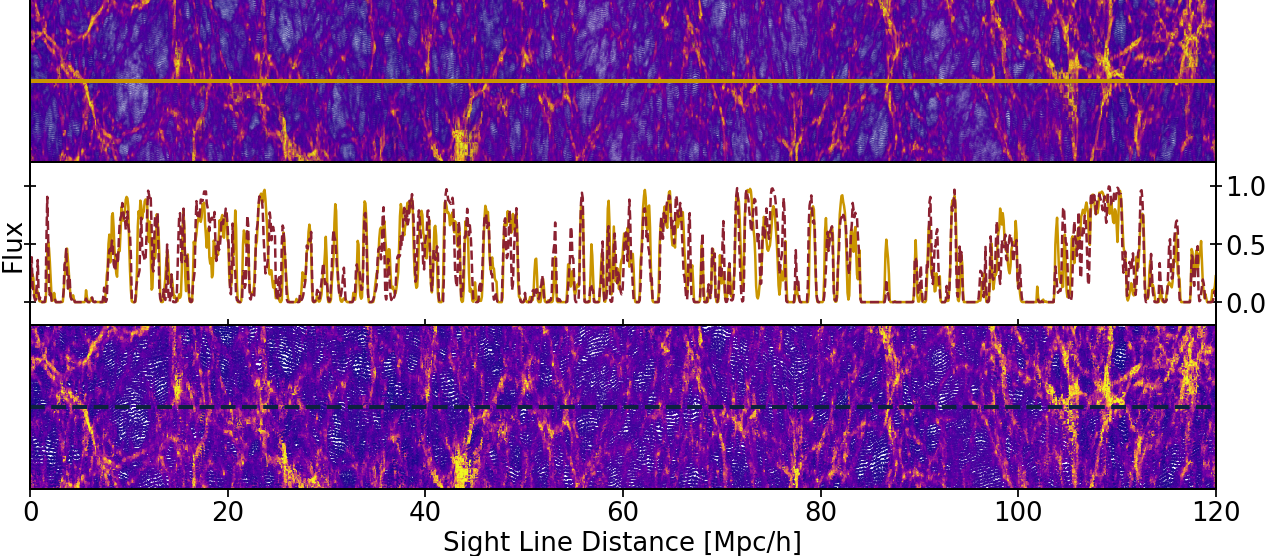
\includegraphics[width=\columnwidth]{figures/spectra_temp_simulation.png}
    \caption{\label{fig:spec_sim}
    Example Lyman-$\alpha$ forest spectra and corresponding gas density and temperature (colors) from an LF and HF simulation at redshift $z=4$.
    The top panel shows high resolution and the bottom panel shows low resolution. The middle panel shows the \lya forest spectra for the skewers passing through the middle of the top panel (high resolution, yellow line) and bottom panel (low resolution, red line).
    }
\end{figure}
The range given for the gas mass resolution is due to the varying value of $h$ in our simulation suite ($\Omega_b h^2$ is fixed, at a value of $0.0224$). We show in Ref.~\cite{2023simsuite} that this gas mass is sufficient for the scales and redshifts probed by the eBOSS flux power spectrum. Our simulations include a full galaxy physics model with star formation, stellar and AGN feedback and inhomogeneous reionization models. Simulations were performed using MP-Gadget\footnotemark, an N-body and smoothed particle hydrodynamics (SPH) code.\footnotetext{\url{https://github.com/MP-Gadget/MP-Gadget}}
MP-Gadget uses the gravitational timestepping algorithm from Gadget-4 \cite{Springel:2021}, and various other algorithmic improvements \cite{2020JCAP...06..002B}.
Simulations are initialised at $z=99$ and finish at $z=2.2$. The galaxy formation model is similar to the \texttt{ASTRID} simulation \cite{2022MNRAS.512.3703B, 2022MNRAS.513..670N} and is described fully in Ref.~\cite{2023simsuite}.

%In \cite{2009MNRAS.398L..26B}, the recommended gas mass resolution for the \lya forest is $2\times10^5$ M$_{\odot}$ h$^{-1}$ at $z=5$ and $1.61\times10^6$ M$_{\odot}$ h$^{-1}$ at $z=2$.
%Our HF simulations have better gas mass resolution than the recommendation for lower redshifts, and slightly worse resolution than recommended at higher redshifts.
%\textbf{However, we include a temperature boost \cite{2019ApJ...874..154D} due to impulsive heating during hydrogen reionization from ionization fronts.
%This increase the thermal free-streaming length at high redshift, which reduces the resolution requirements.}
%Also, we currently restrict our analysis to $z=2.2$ to $z=4.6$, so the recommendation at $z=5$ is more strict than required in this work.

%In \cite{2014JCAP...07..005B}, simulations with box side length of at least $100$ Mpc h$^{-1}$, and a corresponding gas mass resolution of $4.3\times10^5 M_\odot/h$ were recommended for the \lya forest.
%\textbf{Our HF simulations are larger volume than the above recommendation, with slightly lower gas mass resolution.
%In \cite{2014JCAP...07..005B}, they found that simulations run with a similar resolution to our HF samples were no worse than $5\%$ converged.
%When the reduced resolution requirement due to the aforementioned temperature boost is considered, the simulations used in this work simultaneously achieve the volume and resolution recommended in \cite{2014JCAP...07..005B}, without the need for splicing.
%}

\subsection{Cosmological \& Astrophysical Parameters}\label{sec:parameters}

Table~\ref{tab:emulatorparams} summarises the parameters that are varied across our suite of simulations, as well as their limits.
We model the primordial power spectrum $P(k)$ using two parameters: a slope, $n_P$, and an amplitude, $A_P$:
\begin{equation}
    P(k) = A_P \left(\frac{k}{0.78 \mathrm{h/Mpc}}\right)^{n_P - 1}\,.
\end{equation}
We also vary the Hubble parameter $h$, and the total matter density through $\Omega_M h^2$, although we will see these are not strongly constrained by the \Lya~forest. We add three parameters for the He~{\sc ii} reionization model \cite{2020MNRAS.496.4372U}: $z_{Hei}$ and $z_{Hef}$ are the redshifts for the start and end of He~{\sc ii} reionization, and $\alpha_q$ is the quasar spectral index (which scales the peak temperature during He~{\sc ii} reionization).
$z_{Hi}$ is the midpoint redshift of H~{\sc i} reionization.
Finally, $\epsilon_{AGN}$ is the black hole feedback factor, to which the \lya~forest is insensitive.

\begin{table*}
\begin{centering}
  \begin{tabular}{llll}
  \hline
  Parameter & Minimum & Maximum & Description \\
    \hline
    $n_P$  &  $0.8$  & $0.995$ & Scalar spectral index \\
    $A_P$  &  $1.2 \times 10^{-9}$  & $2.6 \times 10^{-9}$ & Power amplitude at $k = 0.78$ h/Mpc \\
    $h$    & $0.65$  & $0.75$ & Hubble parameter \\
    $\Omega_0 h^2$ & $0.14$ & $0.146$ & Total matter density \\
    $z_{Hei}$      & $3.5$  & $4.1$  & Start redshift of HeII reionization \\
    $z_{Hef}$      & $2.6$  & $3.2$  & End redshift of HeII reionization \\
    $\alpha_q$     & $1.3$  & $2.5$ & Quasar spectral index during HeII reionization  \\
    $z_{Hi}$        & $6.5$ & $8$   & Median redshift of HI reionization \\
    $\epsilon_{AGN}$ & $0.03$ & $0.07$ & Thermal efficiency of black hole feedback \\
    $\tau_0$ & $0.75$ & $1.25$ & Mean optical depth at $z=3$ in Eq.~\ref{eq:meanflux}.\\
    $d \tau_0$ & $-0.4$ & $0.25$ & Mean optical depth redshift evolution in Eq.~\ref{eq:meanflux}. \\
    \hline
  \end{tabular}
  \caption{Summary of likelihood function parameters, together with the ranges covered by the emulator. We vary a total of $11$ parameters: $4$ for cosmology, $3$ for the helium reionization model, $1$ for the hydrogen reionization model, $1$ for the strength of AGN feedback and $2$ for the mean optical depth.}
  \label{tab:emulatorparams}
  \end{centering}
\end{table*}

There are two further parameters for the \Lya~effective optical depth, varied by post-processing the artificial spectra. We parametrise the mean flux $\mathcal{F} = \exp(-\tau)$ around the power law redshift evolution from Ref.~\cite{2007MNRAS.382.1657K}, as
\begin{equation}
\tau^{\text{eff}}_{\text{H~{\sc i}}} = 0.0023 \times \tau_0 \times (1+z)^{3.65 + d\tau_0}\,.
 \label{eq:meanflux}
\end{equation}
The parameters varied are $\tau_0$ and $d\tau_0$, with $(1, 0)$ corresponding to the redshift evolution of Ref.~\cite{2007MNRAS.382.1657K}.
As the mean flux is chosen in post-processing, we can dramatically over-sample these parameters. The final set of flux power spectra is thus ten times the number of simulations, or $480$ LF, and $30$ HF simulated flux power spectra. We have freedom to vary the \Lya~mean flux as it is degenerate with the amplitude of the UVB. 

%Note that our emulator construction is designed to easily accommodate more general evolution. Each set of simulated spectra is post-processed at each redshift into ten flux power spectra with a mean flux spread uniformly over a range chosen to include the mean fluxes .

% --------------------------------------------------------------------------------------------------

\subsection{Summary Statistics: Flux Power and IGM Temperature}\label{sec:sim_fps}

%In the companion paper to this work \cite{2023simsuite}, the \lya forest statistics extracted from these simulations are well converged . . .
Figure~\ref{fig:spec_sim} shows an example of the gas density and temperature (colors) at $z=4$ for both high and low resolution in our simulations, demonstrating how spectra connect to the matter density field.
We generate a total of $3\times 480^2 = 691,200$ spectra from each snapshot of each simulation, from $z=4.6$ to $z=2.2$ in increments of $\Delta z=0.2$, with a pixel resolution of $10$ km s$^{-1}$.
We generate \lya forest absorption spectra using Fake Spectra Flux Extractor \cite{2017ascl.soft10012B}\footnotemark, described in \cite{2015MNRAS.447.1834B}.
\footnotetext{\url{https://github.com/sbird/fake_spectra}}
We compute the 1D flux power spectrum of the \Lya~forest flux, averaged over all sightlines. The flux power is defined as 
\begin{equation}
 P_F(k) = |L^{-1}\tilde{\delta}^2_F(k)|\,.   
\end{equation}
$\tilde{\delta}^2_F(k)$ is the Fourier transform of the flux excess, $\delta_F(k) = F(k)/\langle F(k) \rangle - 1$, and $L$ is the length of the sightline. 

Our simulations contain a realistic population of DLAs, which we mask as in the observational pipeline. We extract the IGM mean temperatures directly from the simulation snapshots. First, the temperature and density for all the gas particles in the simulation are retrieved, then all particles that are within $5\%$ of the critical density are retained. The median temperature of these retained particles is used as the IGM mean temperature. All of the \lya forest flux power spectra, IGM mean temperatures, trained emulators, as well as select MCMC chains are available at: \url{https://github.com/mafern/InferenceLyaData}.

%
% Figure~\ref{fig:sim_fps} shows flux power spectra from all the LF (blue, solid) and HF (gold, dashed) simulations at several redshifts.
% Shown below each redshift panel in red are the ratios of the flux power spectra for simulations that were run at both resolutions.
% Note that there are ten times more flux power spectra shown here than simulations, due to the previously discussed post-processing method of mean flux rescaling.
%
% \begin{figure}
%     \centering
%     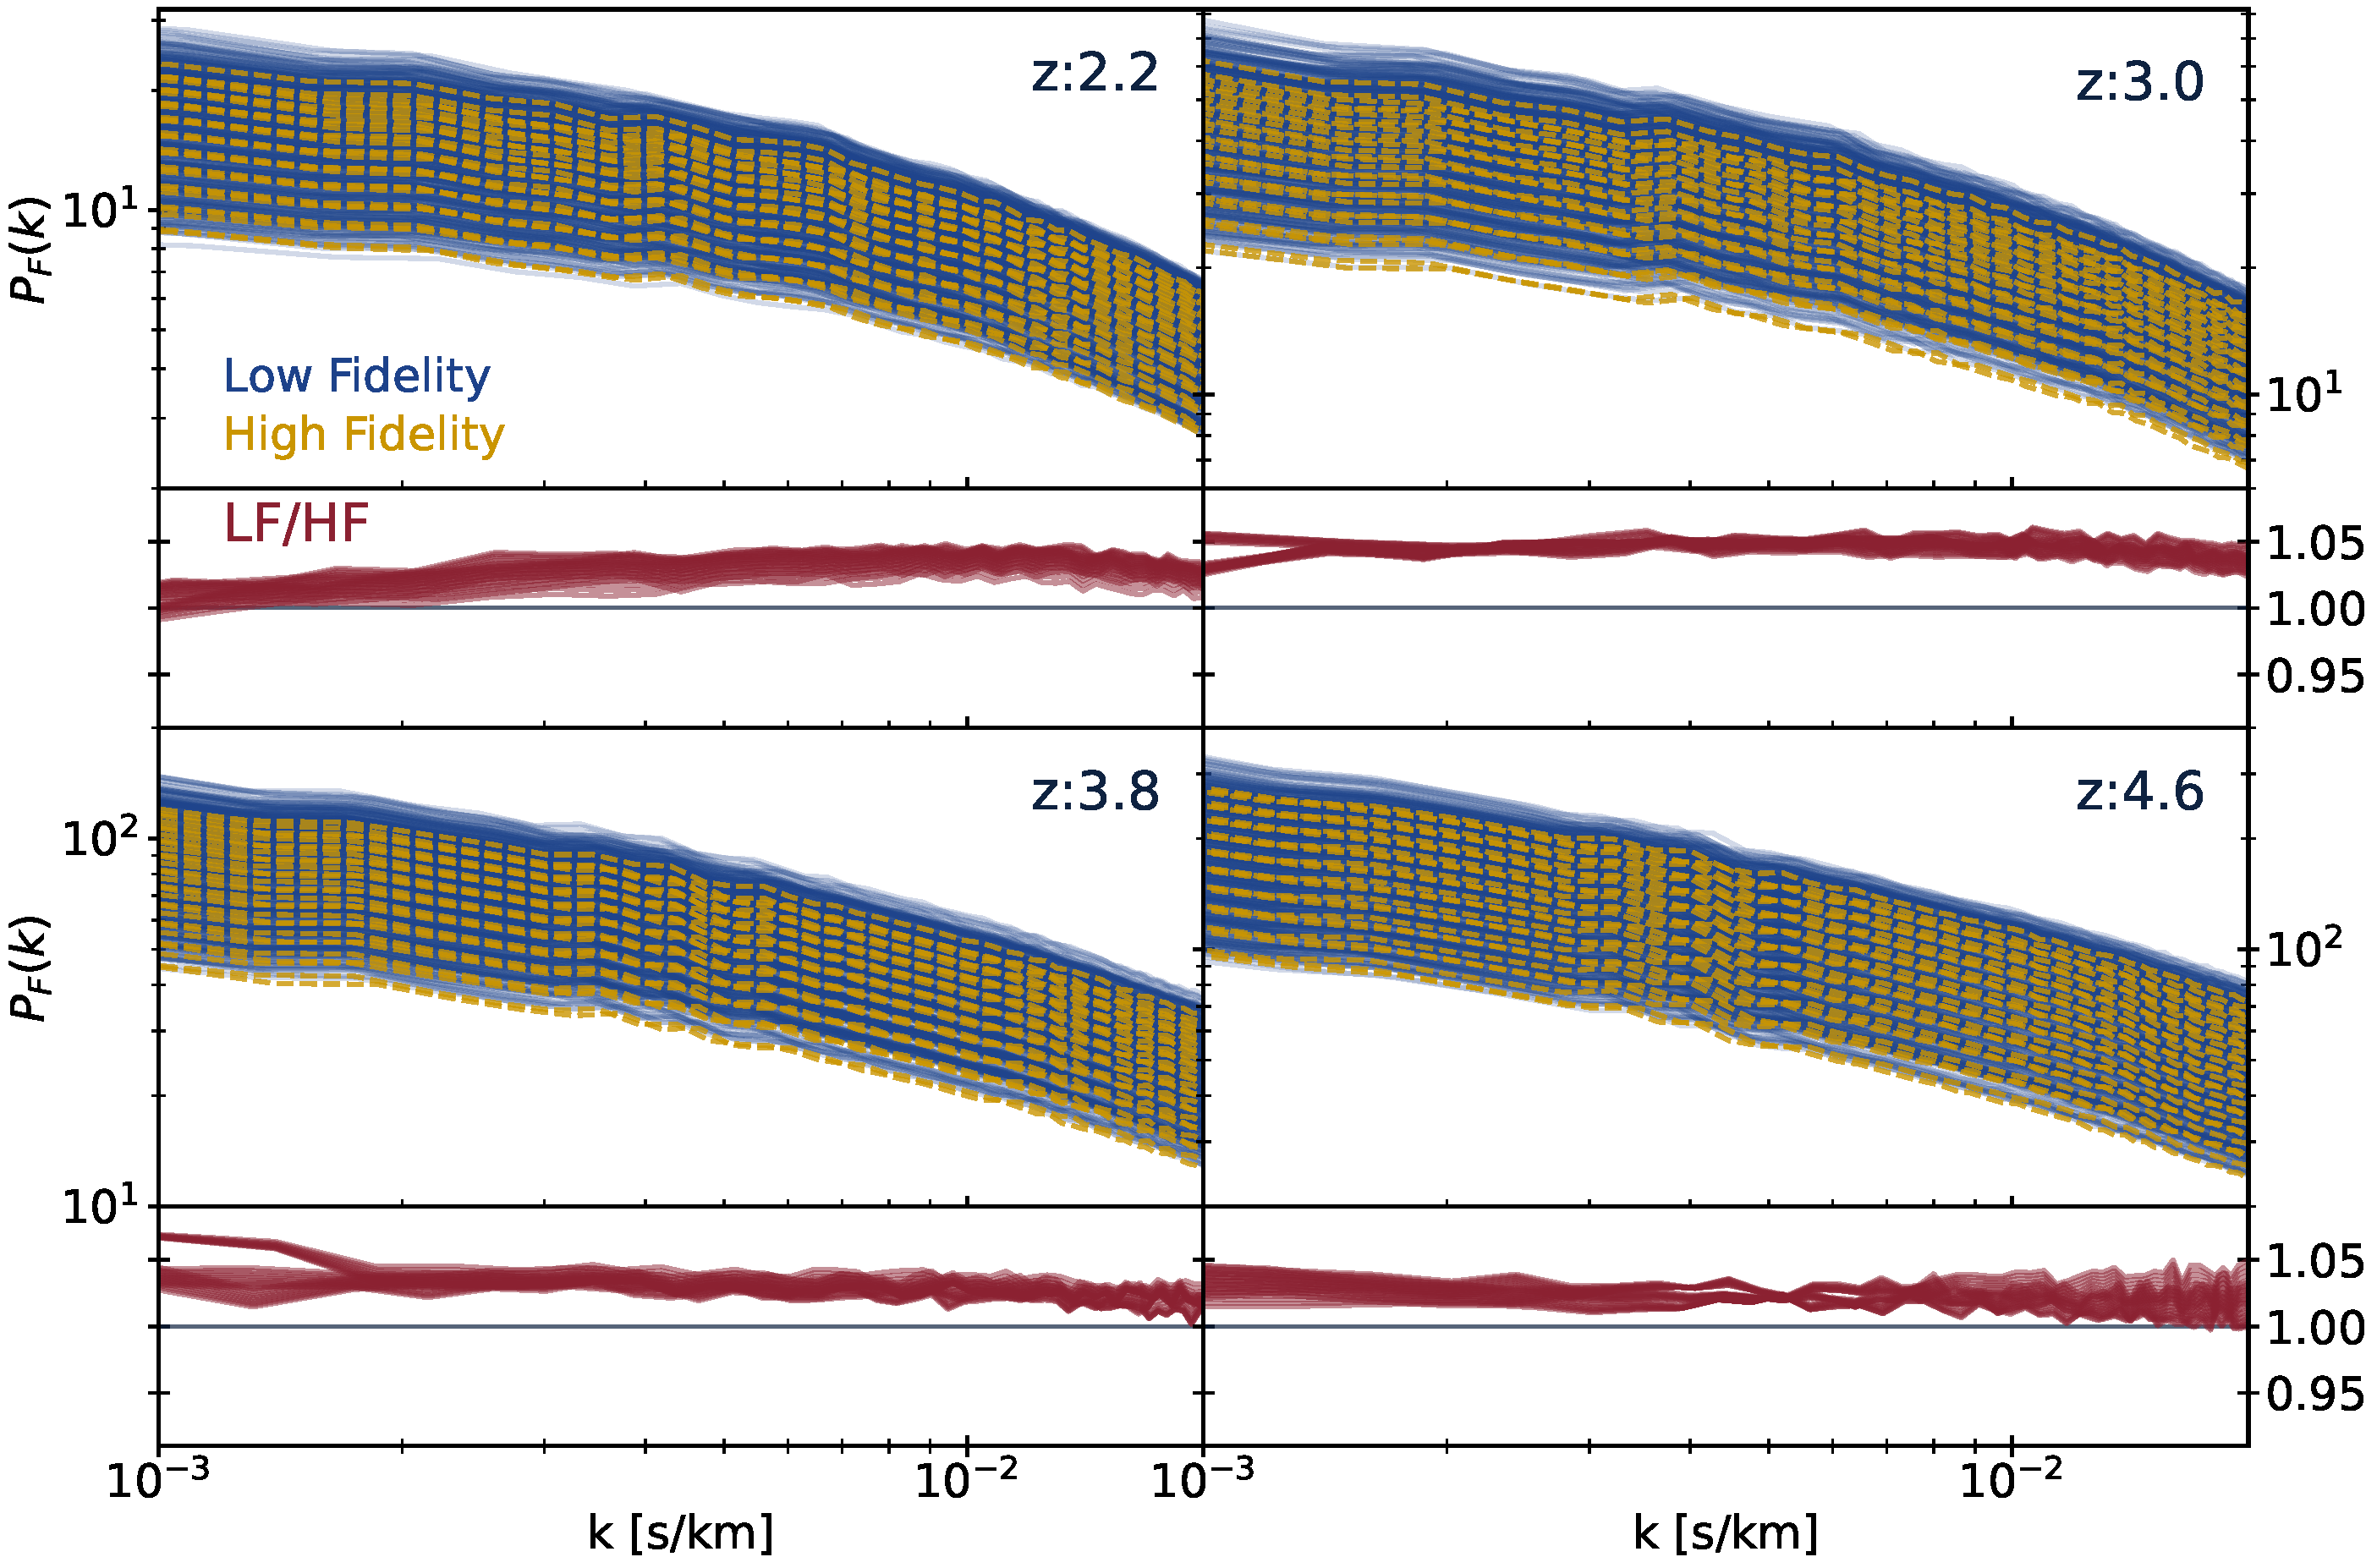
\includegraphics[width=\textwidth]{figures/fluxpower_comp.pdf}
%     \caption{\label{fig:sim_fps}
%     Flux power spectra from all LF (blue, solid) and HF (gold, dashed) simulations at $z=2.2$, $z=3.0$, $z=3.8$, and $z=4.6$.
%     In each panel below the flux power, the ratio of the flux power spectra for simulations run at both resolutions is shown, $LF/HF$.}
% \end{figure}

% --------------------------------------------------------------------------------------------------


% \begin{figure}
%     \centering
%     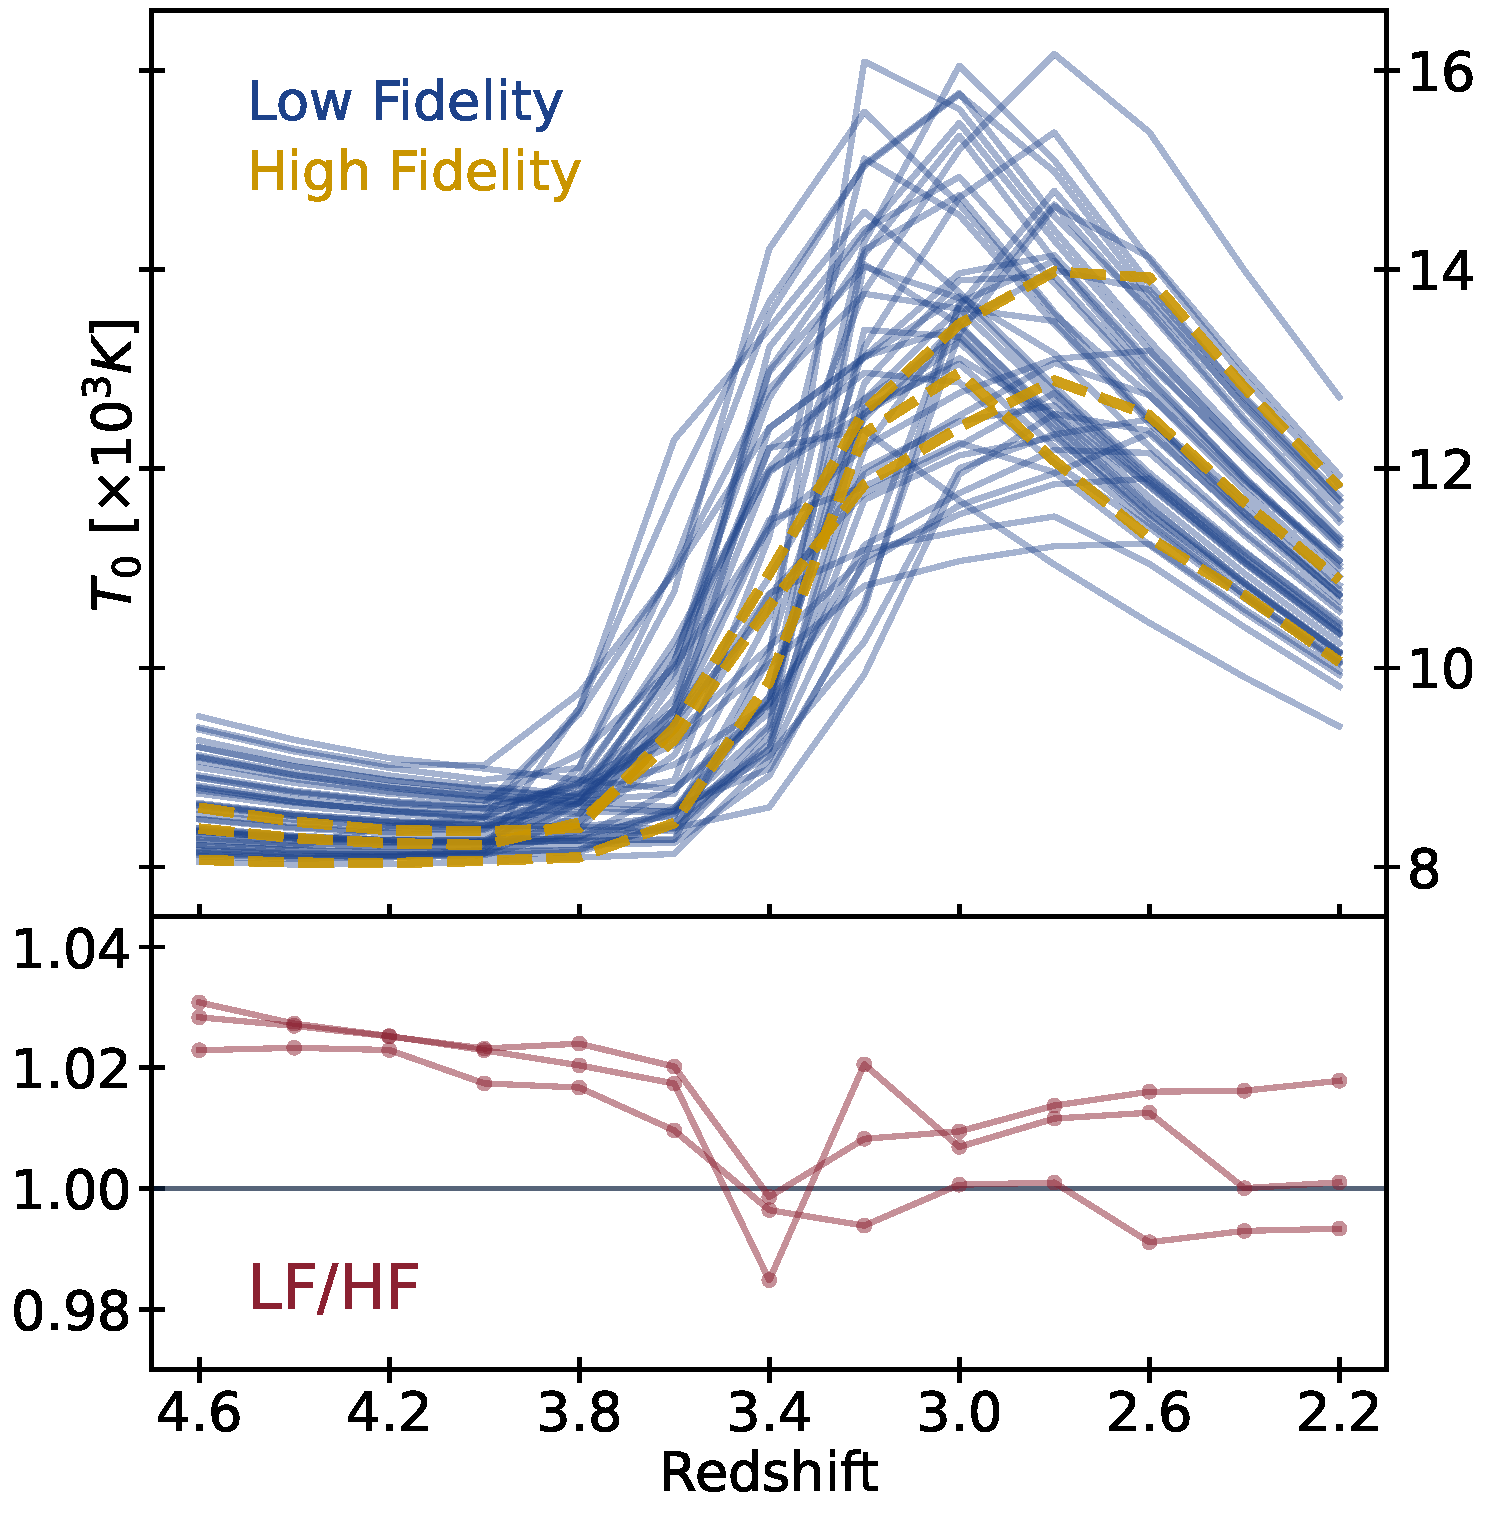
\includegraphics[width=0.66\textwidth]{figures/meant_range.pdf}
%     \caption{\label{fig:sim_temp}
%     IGM mean temperatures from all LF (blud, solid) and HF (gold, dashed) simulations for the full redshift range.
%     The bottom panel shows the ratio of the mean temperatures from simulations that were run at both resolutions, $LF/HF$.}
% \end{figure}

%--------------------------------------------------------------------------------------------------
% --------------------------------------------------------------------------------------------------
% --------------------------------------------------------------------------------------------------
% --------------------------------------------------------------------------------------------------
% --------------------------------------------------------------------------------------------------

\subsection{Gaussian Process Emulators}\label{sec:gps}

We use the Gaussian Process emulators described in Refs.~\cite{2022MNRAS.517.3200F, 2023simsuite} for the 1D flux power spectra and mean IGM temperature extracted from our simulations. The emulators interpolate over simulation outputs and make predictions for arbitrary parameter sets within the parameter limits shown in Table~\ref{tab:emulatorparams}. We use a multi-fidelity model, which allows simulations with different particle loads, and thus costs, to be combined together.
%This allows construction of an emulator that is a good approximation to a high fidelity model, but with most of the parameter space covered by cheaper, low fidelity simulations.
%makes full use of the range of scales and redshifts probed by \lya forest observations, at a significantly reduced computational cost.
%, as  (e.g. each HF simulation requires approximately sixteen times more node-hours to run than an LF simulation).
Specifically, we combine simulations run at two different resolutions, high fidelity (HF) and low fidelity (LF) specified in Table~\ref{table:simulations}. The multi-fidelity prediction for the HF outputs (shown here for the \lya forest flux power spectrum, but equally valid for the mean temperature) is given by a linear multi-fidelity model:
\begin{equation}
    P_F^{^\mathrm{HF}}(k, \boldsymbol{\theta}) = \rho(k) \cdot P_F^{^\mathrm{LF}}(k, \boldsymbol{\theta}) + \delta(k, \boldsymbol{\theta}),
    \label{eq:ko_model}
\end{equation}
where $\rho$ is a cosmology-independent but scale-dependent parameter, and $\delta(k, \boldsymbol{\theta})$ is a GP (independent of the LF output), both of which are optimized using the training samples.
%Since $\rho(k)$ is a multiplicative correction, and $\delta(k, \boldsymbol{\theta})$ is an additive correction,
% This is often called a linear multi-fidelity model.
We implement our multi-fidelity models using Emukit \cite{2021arXiv211013293P}.

Ref.~\cite{2023simsuite} quantifies the accuracy of our emulator using a leave-one-out technique, in which one simulation is chosen as a `left out' sample. A smaller emulator built excluding all samples from this simulation is used to predict the summary statistic for the left out sample. After computing leave-one-out interpolation errors for all potential test samples, we found on average $0.2\%$ accuracy for the low-fidelity simulations and $1\%$ for the high fidelity simulations. The last is likely a significant over-estimate of the actual error since the leave-one-out procedure in this case is missing $1/3$ of the total training data. The emulator accuracy indicates that the emulators are performing well, with potential errors significantly smaller than the 7\% average uncertainty in mean IGM temperature measurements \cite{2019JCAP...07..017C}.
Our likelihood function and emulator code is publicly available\footnote{\url{https://github.com/sbird/lya_emulator_full}}.

%Gaussian processes \citep{2006gpml.book.....R} are a trainable method for providing function prediction in a Bayesian framework.
%In this case, the GP is used to interpolate simulation outputs as a function of the simulation input parameters that are varied in the training samples (see Figure~\ref{fig:samples}).
%In a Gaussian process, a distribution of functions is learned through the training samples (simulation input/output pairs), and the mean of the learned distribution serves as the prediction, while the variance of the distribution quantifies the prediction uncertainty.
%\textbf{This allows a prediction to be cheaply produced for arbitrary simulation inputs (within the parameter space of the training samples -- GPs work poorly for extrapolation).}
%We use the GPy \cite{gpy2014} package to implement Gaussian processes within our emulator model.
%
% If $P_F(\boldsymbol{\theta})$ is the simulated \lya forest flux power spectrum (the following also applies to the IGM mean temperature, $T(\boldsymbol{\theta})$) as a function of $\boldsymbol{\theta}$, the input parameters to the simulation, then we are modeling this output as draws from a learned distribution,
% \begin{equation}
%     P_F(\boldsymbol{\theta}) \sim GP(\mu(\boldsymbol{\theta}), k(\boldsymbol{\theta}, \boldsymbol{\theta}^{\prime})),
% \end{equation}
% where $\mu(\boldsymbol{\theta})$ and $k(\boldsymbol{\theta}, \boldsymbol{\theta}^{\prime})$ are the mean and covariance function for the distribution, respectively.
% As in \cite{2022MNRAS.517.3200F}, we rescale the training samples by their median (the LF median for both single- and multi-fidelity emulators) so that we may assume a zero mean function during the GP training.
% The predictions are then multiplied by this rescaling factor to produce sensible predictions.
% With a zero mean function, it only remains for the covariance function to be trained, which amounts to selecting a covariance kernel and training the free parameters of that kernel.
% Here, as in \cite{2022MNRAS.517.3200F}, we use the sum of a radial basis function (RBF) kernel and a linear kernel to model our outputs.
%
% The total kernel (RBF + linear kernels) is given by:
% \begin{equation}
%         k_\mathrm{RBF}(\boldsymbol{\theta}, \boldsymbol{\theta}'; \sigma_0, \boldsymbol{l}) + k_\mathrm{LIN}(\boldsymbol{\theta}, \boldsymbol{\theta}'; \boldsymbol{\sigma})\\
%         = \sigma_0^2 \exp{\left( \sum_{i=1}^{d} -\frac{(\boldsymbol{\theta}_i - {\boldsymbol{\theta}_i}')^2}{2 l_i^2} \right)} +  \sum_{i=1}^{d} \sigma_i^2 \boldsymbol{\theta}_i {\boldsymbol{\theta}_i}',
% \end{equation}
% where $d$ is the dimensionality of the input parameters.
% The hyperparameters that are learned from the training samples are: variances for the RBF ($\sigma_0^2$) and  linear ($\boldsymbol{\sigma}^2$) kernels, and the lengthscale controlling the smoothness of the RBF kernel, $\boldsymbol{l}$.
% The RBF lengthscale and linear variance hyperparameters are shown as vectors here, indicating that an independent value is assigned for each dimension $d$ of the input for each of these hyperparameters.
% This is called Automatic Relevance Determination (ARD), and we use this in all cases for the LF \lya forest flux power spectrum.
% Including ARD allows the GP to train a separate hyperparameter for each dimension of the input, such that dimensions that have a more sensitive effect on the prediction can be given a smaller scale, e.g. the effect of $A_p$ on the mean temperature is negligible, while $\alpha_q$ has a large effect.
% For the IGM mean temperature GP, we only use ARD for the RBF kernel.
% Unlike for the flux power predictions, including ARD for the linear variance hyperparameter had no effect on the accuracy of the mean temperature predictions.
%
% The prediction and predicted uncertainty for a Gaussian process come from the mean and variance of the learned distribution, and can be written as the following closed-form expressions (for a full derivation, see \cite{2006gpml.book.....R}):
% \begin{equation}
%     \begin{split}
%         \mu(\boldsymbol{\theta}) &= \boldsymbol{\mathrm{K}}(\boldsymbol{\theta}, \mathcal{D})^\intercal \boldsymbol{\mathrm{K}}(\mathcal{D})^{-1} \boldsymbol{P_F}(\mathcal{D}); \\
%         \sigma^2(\boldsymbol{\theta}) &= k(\boldsymbol{\theta}, \boldsymbol{\theta}) - \boldsymbol{\mathrm{K}}(\boldsymbol{\theta}, \mathcal{D})^\intercal \boldsymbol{\mathrm{K}}(\mathcal{D})^{-1} \boldsymbol{\mathrm{K}}(\boldsymbol{\theta}, \mathcal{D}).
%     \end{split}
% \end{equation}
% where $\boldsymbol{\theta}$ are the new inputs for which a prediction is desired, $\mathcal{D}$ is the vector of training inputs, $\boldsymbol{P_F}(\mathcal{D})$ ($\boldsymbol{T}(\mathcal{D})$ for the mean temperature) is the vector of training outputs, $\boldsymbol{\mathrm{K}}(\mathcal{D})$ is the training data covariance matrix, and $\boldsymbol{\mathrm{K}}(\boldsymbol{\theta}, \mathcal{D})$ is the vector of covariances between the training data and new inputs.

% --------------------------------------------------------------------------------------------------
% --------------------------------------------------------------------------------------------------